\documentclass[paper-main.tex]{subfiles}


\begin{document}
% I've rephrased the first part of this section a lot and provide some justification below
% I think we need to lead with the details of the signal here (similar to the last section), not the specifics of the data analysis as the issues seem confused here. The fact that long data sets are analysed is not because of the signal wandering, if anything that's an argument against analysing long data sets to make detection easier, it's because the signal has low amplitude. Also what is the justification of the "(but not always)" statement, do you have a reference? - hannah


\begin{comment}
Continuous wave searches, such as in Refs.~\cite{SuvorovaEtAl:2016,SuvorovaEtAl:2017,SearchTwoSpecS6:2017,SunEtAlSNR:2018,JonesSun:2020}, are often (but not always) performed on long datasets (months to years in duration). 
The frequency of a continuous wave signals may wander significantly over this timescale, due to stochastic internal processes in the superfluid interior of isolated neutron stars~\cite{MelatosDouglassSimula:2015,Jones:2010} or variable accretion flows onto a neutron star from a stellar companion (e.g. as in LMXBs)~\cite{BildstenTB:1998}. In this context, wandering ``significantly'' means ``across multiple frequency bins'', where the typical width of a frequency bin is the reciprocal of the total observing time~\cite{JKS:1998,ScoX1O2Viterbi:2019}.
The audio analogue to these continuous wave signals is a tone that wanders in frequency; a note that changes pitch. Here, we adapt the data analysis technique used to search for slowly wandering continuous waves signals from spinning neutron stars in aLIGO and aVirgo data~\cite{SuvorovaEtAl:2016,SuvorovaEtAl:2017}. 
\end{comment}


Unlike the signal considered in Section~\ref{sec:single_tone}, continuous gravitational-waves may not be monochromatic.
A continuous-wave signal may wander slowly (and randomly) in frequency over time, due to stochastic internal processes in the superfluid interior of isolated neutron stars\cite{MelatosDouglassSimula:2015,Jones:2010}, or variable accretion flows from a stellar companion for neutron stars in binaries as in LMXBs~\cite{BildstenTB:1998}. 
The audio analogue is a tone that wanders in frequency: a note that changes in pitch. 



A Fourier transform applied to the whole dataset (as in Section~\ref{todo}) is not well suited to the wandering frequency case, as the signal can be spread across multiple frequency bins making it challenging or perhaps impossible to detect. 
%A different means of detection is needed for a signal which has a randomly wandering frequency. 
The analysis techniques used in this section are inspired by those used to search for continuous waves from spinning neutron stars in LIGO and Virgo data~\cite{SuvorovaEtAl:2016,SuvorovaEtAl:2017}. 
Continuous-wave searches are performed on long datasets, months to years in duration. 
The frequency of the signal can wander significantly over the observation period. 
In this context, ``significantly'' means across multiple frequency bins, where the typical width of a frequency bin is the reciprocal of the total observation time~\cite{JKS:1998,ScoX1O2Viterbi:2019}.
One method to search for a wandering signal is to split the timeseries data into several shorter segments which are analysed individually.%, and then recombine them under some continuity assumption to coherently analyse the whole set. 
% I think the following is more accurate. The antenna beam pattern is used to compute a detection statistic. Which detection statistic to use depends on the type of target. -Hannah

A ``detection statistic'' is used to quantify the likelihood of a signal being present in the data at each frequency and timeseries segment. 
In gravitational-wave data analysis, the detection statistic gives the likelihood of a signal given the antenna beam pattern of the detector, which varies as the Earth rotates and orbits the Sun~\cite{JKS:1998}. 
%Most continuous wave searches use detection statistics to quantify the likelihood of a signal being present in the data at each frequency for each timeseries segment. 
%The detection statistic used depends on the antenna beam pattern of the detector, which varies as the Earth rotates and orbits the Sun, and the type of target~\cite{JKS:1998,SuvorovaEtAl:2017}.
The choice of detection statistic used depends on the type of target~\cite{JKS:1998,SuvorovaEtAl:2017}.
In this work, we take the discrete Fourier transform of each timeseries segment and use its amplitude at each frequency as a detection statistic.
This maximises the likelihood of detecting a sinusoidal signal in Gaussian noise, as described in Appendix~\ref{app:sinusoid_likelihood}. 
The detection statistic is normalised for convenience and we use it to form a grid in time and frequency (a spectrogram) which displays the frequency content of the signal over time. 
% moved one sentence up 
%We also normalise the detection statistics for convenience.


Following the method of Refs.~\cite{SuvorovaEtAl:2016,SuvorovaEtAl:2017}, we use a hidden Markov model to recover the wandering signal from noisy data. 
In a Markov process, the current state depends only on the previous state (in this case the state is the frequency of the signal). 
In a hidden Markov model, the frequency state of the signal is unknown, or hidden, and can undergo transitions at discrete times. 
%To do this, we define the frequency of the signal as a hidden (unknown) state which can undergo transitions at discrete times. 
The transitions are Markovian in that the hidden state (i.e.\ frequency) of the system at any time depends solely on its state at the previous time. The detection statistic (observable) relates the hidden states of the system to the observed data.
The Viterbi algorithm~\cite{Viterbi:1967} is used to find the most probable sequence of states given the sequence of observables.
%To perform the task of recovering the signal, we use the Viterbi algorithm~\cite{Viterbi:1967} to efficiently find the most probable path through the spectrogram given the sequence of observations.
This method is used in continuous-wave searches for a variety of astrophysical targets~\cite{ScoX1O2Viterbi:2019, ScoX1ViterbiO1:2017, MillhouseStrangMelatos:2020, JonesSun:2020, MiddletonEtAlO2LMXBs:2020, PostMergerRemnantSearch:2019, SunEtAlSNR:2018, viterbi_application} and forms the basis of the analysis in this section. 
 

In Section~\ref{sec:viterbi} we review the Viterbi algorithm and its application to this work. 
In Section~\ref{sec:wanderingResults} we present results for recovery of a wandering frequency audio signal. 






\subsection{The hidden Markov model and Viterbi algorithm}
\label{sec:viterbi}


We use the schematic in Fig.~\ref{fig:viterbi} to aid our explanation of the method. 
It represents a spectrogram with $N_t$ time bins and $N_f$ frequency bins. 
We label the elements of the time and frequency  grid as $t_i$ and $f_j$ respectively, where $i=0,1,2,...N_t$ and $j=0,1,2,...,N_f$. 
We use the normalised Fourier amplitude $F(t_i,f_j)$ as the detection statistic, which is represented by the shading of each grid point (lighter corresponds to higher value). 


%The spectrogram schematic, as shown in Fig.~\ref{fig:viterbi}, has $N_t$ time and $N_f$ frequency bins. 
%We label the elements of the time and frequency  grid as $t_i$ and $f_j$ respectively, where $i=0,1,2,...N_t$ and $j=0,1,2,...,N_f$. 
%The normalised Fourier amplitude $F(t_i,f_j)$ is the detection statistic. 


The objective is to find the most likely path through the grid given the observed data and any probabilistic constraints on how the frequency of the signal can wander from $t_i$ to $t_{i+1}$. 
In continuous wave searches, a physical model of the target informs how far the frequency of the signal can wander over at each time. 
This information is encoded in the transition probability matrix $A(f_k,f_m)$, which describes the probability of system transitioning from state $f_i$ at $t_i$ to a state $f_{j}$ at $t_{i+1}$. 
Here, we allow the frequency of the signal to either (a) stay in the same bin; (b) move up by a single frequency bin; or (c) move down by a single frequency bin at each transition. 
The possible transitions are shown as lines in Fig.~\ref{fig:viterbi}.
We assign these three transitions equal probability, i.e.\ $A(f_k,f_m)=1/3$ for $k=m+1,m,m-1$ and $A(f_k,f_m)=0$ otherwise.



We define the probability of the system having frequency $f_j$ at the initial time $t_0$ to be equal to the (normalised) detection statistic at that state (i.e.\  ${\rm Pr}[f(t_0) = f_j] = F[t_0,f_j]$).
The probability of the system having frequency $f_j$ at any later time $t_{i+1}$ is then defined recursively by
\begin{eqnarray}
{\rm Pr}[f(t_{i+1})=f_j] =~& F[t_{i+1},f(t_{i+1})] \nonumber \\
                     &\times A[f(t_{i+1}),f(t_i)]  \nonumber \\
                     &\times {\rm Pr}[f(t_i)].
\label{eqn:recursiveViterbi}
\end{eqnarray}
for any path through the grid. 
The sequence $f(t_0),f(t_1),\dots,f(t_{N_t})$ that maximizes ${\rm Pr}[f(t_{N_t}) = f_j]$ is the optimal Viterbi path terminating in the frequency bin $f_j$. 
We can then maximize the latter quantity over $0 \leq j \leq N_f$ to find the optimal Viterbi path overall, i.e. terminating in any frequency bin. 


The Viterbi algorithm provides a computationally efficient method for finding the optimal path. 
At every $t_i$ all but $N_f$ possible paths are eliminated (see also Ref.~\cite{ScoX1ViterbiO1:2017}). 
Here we describe the algorithm in pseudocode while referring to the schematic in Fig.~\ref{fig:viterbi}.%, where the circles indicate the elements in the spectrogram with the lighter colours corresponding to a higher likelihood. 
The implementation used in this work is available online (see Appendix~\ref{app:code}).
\begin{enumerate}
\item Starting at time $t_1$, each $f_j$ state can originate from three prior states at time $t_0$ (except for $f_0$ and $f_{N_f}$ which only have two). The paths between these states are indicated by the lines in Fig.~\ref{fig:viterbi}. At each $f_j$ state, we select the path with the highest $A[f(t_0),f(t_1)] {\rm Pr}[f(t_0)]$ value as the most probable path. These choices are highlighted using the black lines in Fig.~\ref{fig:viterbi} while the grey lines show the rejected paths. For example, the most probable connection to the element labelled (a) is the one directly behind it (i.e., $f_4$). Therefore, this path is selected as the best path from $t_0$ to $t_1$ for $f_4$. To allow backtracking at the end, the index of the most probable connection to a node along with the value of the best path to that node is stored, for each node.

\item Moving to time $t_2$, again, we select the path which maximises the recursive quantity in Eqn.~\ref{eqn:recursiveViterbi} for each $f_j$. These are again shown by the solid black lines between the nodes at $t_1$ and $t_2$ in Fig.~\ref{fig:viterbi}.

\item Step 2 is repeated until the end of the grid ($t=t_{N_t}$) is reached with only the best paths being stored at each iteration. 

\item Each state $f_j$ at $t=t_{N_t}$ has some value ${\rm Pr}[f(t_{N_t})=f_j]$ (Eqn.~\ref{eqn:recursiveViterbi}), which represents the probability of the most likely path that ends in state $f_j$ at $t_{N_t}$. The Viterbi algorithm then selects the terminating frequency bin $f(t_{N_t})$ with the highest probability, marked by (b) in Fig.~\ref{fig:viterbi}.

\item The last step is to find the Viterbi path (the overall best path that terminates in the frequency bin with the highest probability in step 4). The Viterbi path is found by backtracking along the stored best connections at each $t_i$ (see also Appendix~\ref{app:viterbi}). In Fig.~\ref{fig:viterbi}, we see that the path ending at (b) started at (c) and is highlighted in orange.
%\item The Viterbi path (the overall best path) is then found by backtracking along the stored best connections at each $t_i$ (see also Appendix~\ref{app:viterbi}). In Fig.~\ref{fig:viterbi}, we see that the path ending at (b) started at (c) and is highlighted in orange.
\end{enumerate}

In the following section, we use the Viterbi algorithm to recover a slowly wandering signal.


% The Viterbi algorithm is an example of a dynamical programming algorithm, where a computation can be broken down into a series of sub-computations.
% The Viterbi path for a time series sequences spanning $t_0$ to $t_{N_t}$ contains the Viterbi path for sub-sequences of that time series. 
% The algorithm is computationally efficient, at every time step all but $N_f$ possible paths are eliminated (see also Ref.~\cite{ScoX1ViterbiO1:2017}).

\begin{figure}
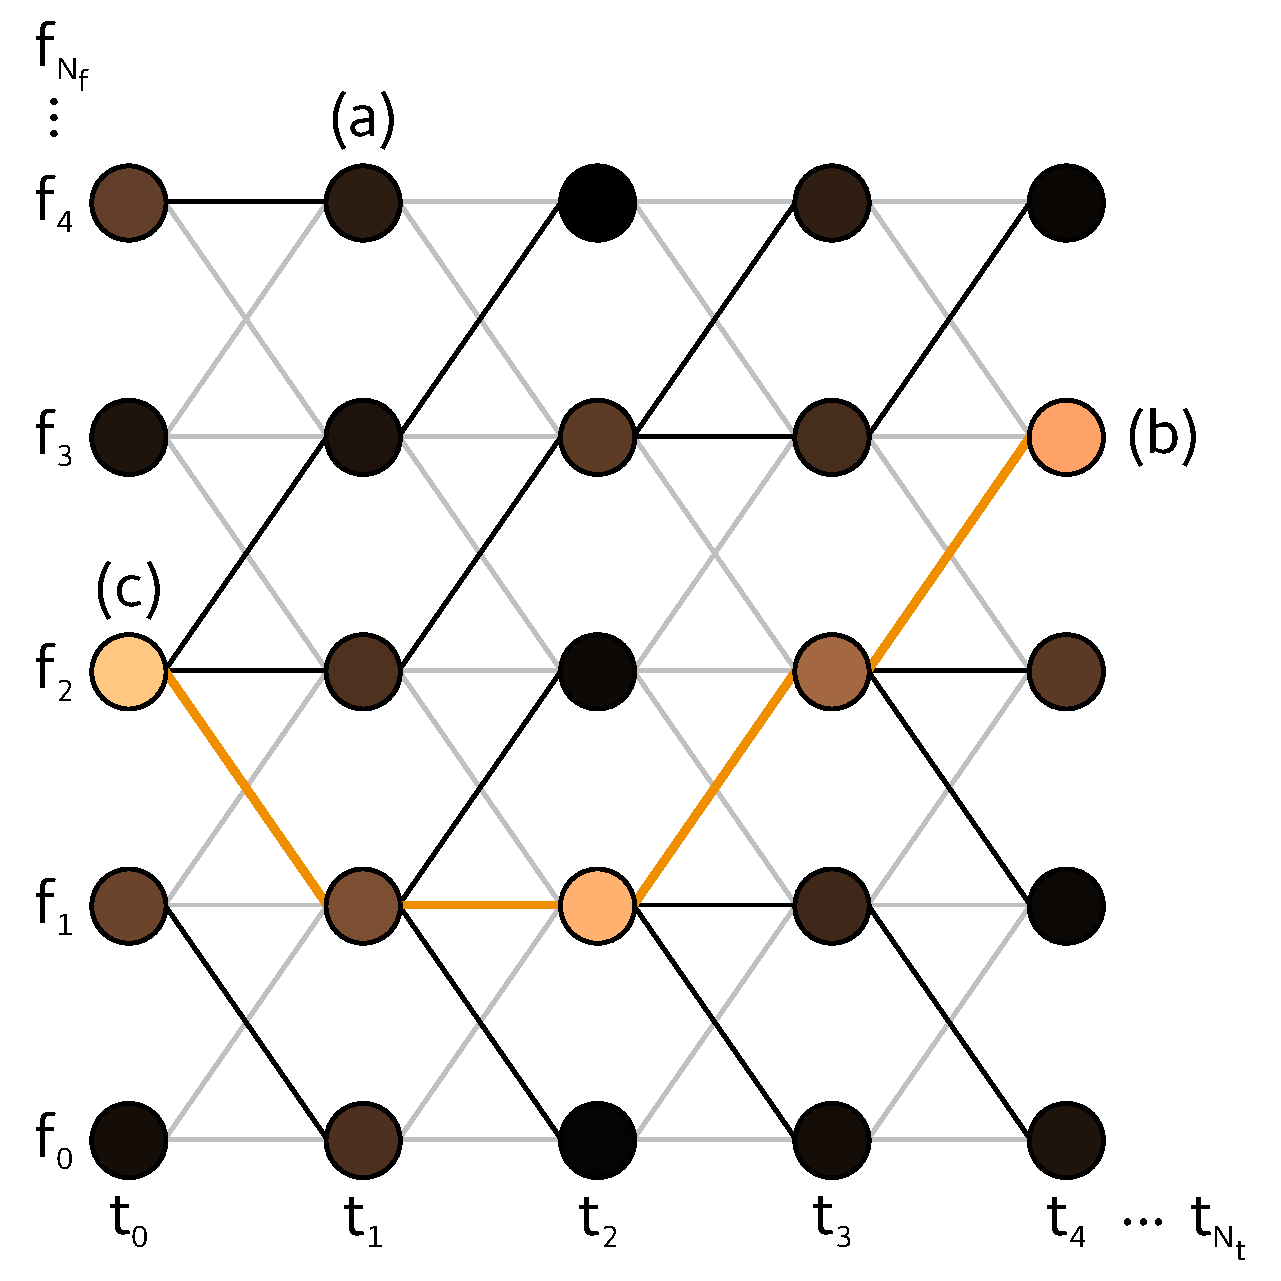
\includegraphics[width=0.49\textwidth]{figures/viterbiDiagram.pdf}
\caption{\label{fig:viterbi}
A schematic diagram of the Viterbi algorithm. 
Each circle represents an element in the time-frequency grid starting from the instant $t_0$ on the left and ending at $t_{N_t}$ on the right. 
Vertically, the grid starts from frequency $f_0$ at the bottom and ending at $f_{N_f}$ at the top. 
The colour of each circle indicates the likelihood that a signal is present in the box, where a lighter colour corresponds to a higher likelihood. 
At each time, the paths can move up one $f$ bin, move down one $f$ bin, or stay at the same $f$ bin (shown by lines in the diagram). 
Each circle has three paths leading to it, indicated by the lines. 
The best path to each circle at each $t_i$ is highlighted in black. 
Some routes through the grid are found to be dead ends, with respect to optimally reaching the other side, such as the path ending at $t_1$ marked (a). 
At $t=t_{N_t}$ the algorithm chooses the terminating frequency circle which has the highest value given by Eqn.~\ref{eqn:recursiveViterbi}, marked (b). 
The Viterbi path is the path leading to this circle, highlighted in orange from (b) to the start at (c). 
}
\end{figure}



\subsection{Wandering frequency results}
\label{sec:wanderingResults}

\begin{figure*}
	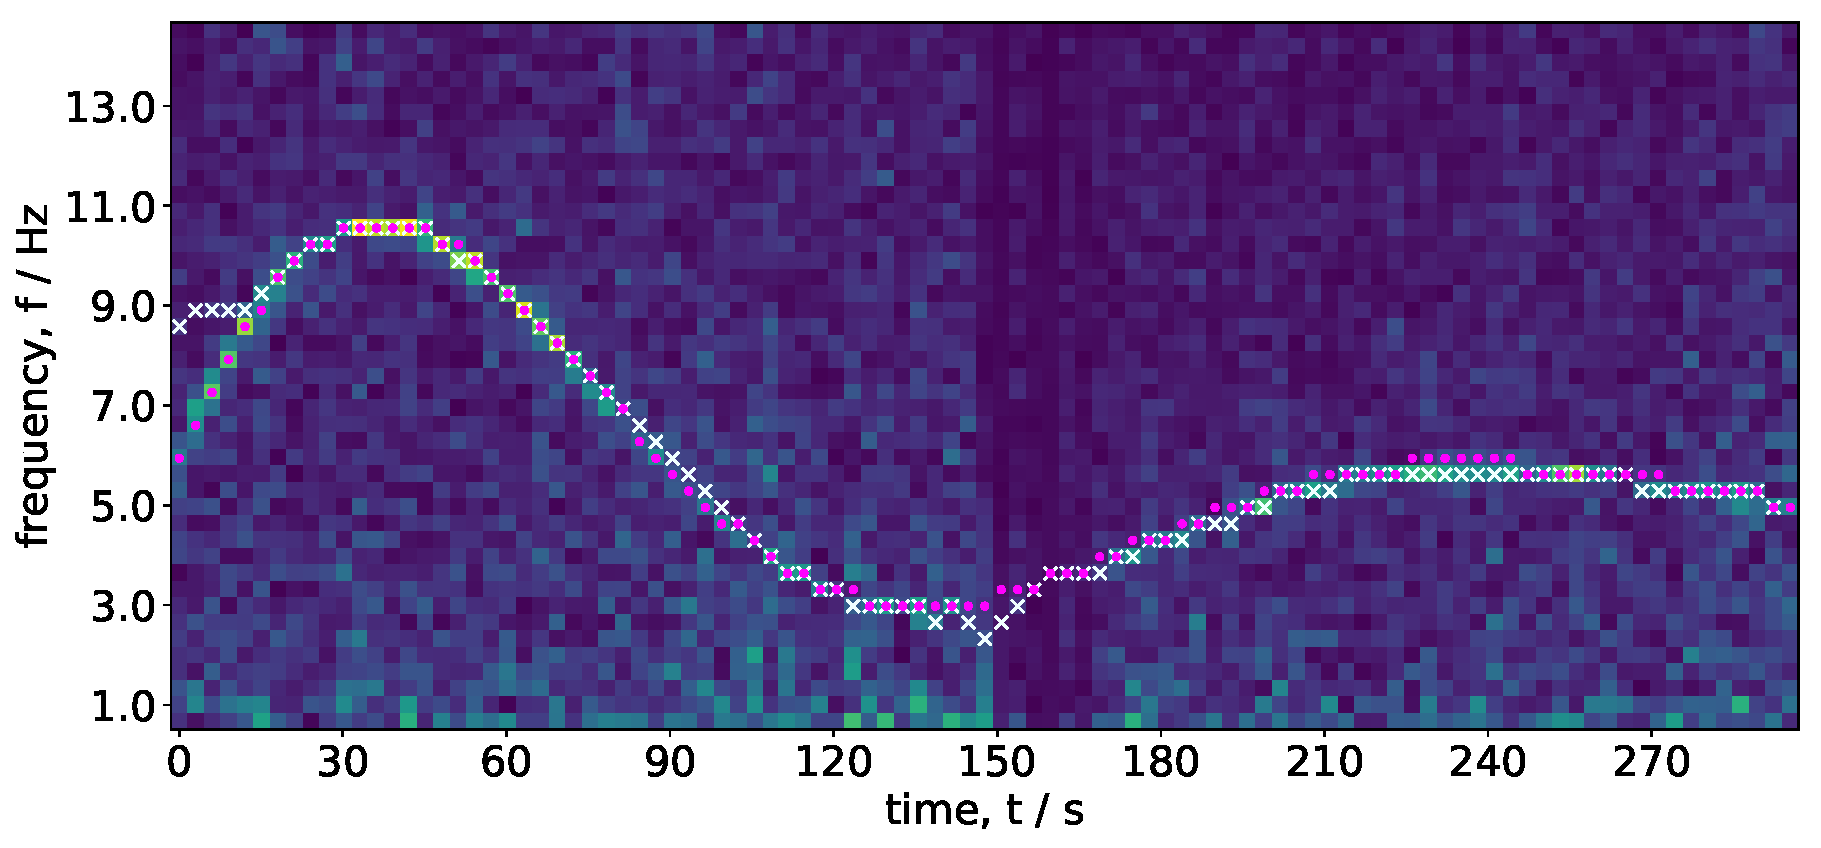
\includegraphics[width=\textwidth]{figures/expt_overlay_2_viterbi_test_webcam.pdf}
	\caption{\label{fig:viterbi_overlay}
Recovery of a wandering tone using the Viterbi algorithm. 
The spectrogram shows the observed frequency (Fourier) amplitude in each time-frequency bin. 
The overlaid pink-dot and white-cross markers show the injected signal and recovered Viterbi path, respectively. 
On the left, before $\sim 15\,{\rm s}$, the signal changes frequency too quickly for the Viterbi algorithm to recover, given a parameter for the rate of change of one frequency bin per time bin. 
At $150\,{\rm s}$ the data appears anomalous, which may be due to some background noise. }
\end{figure*}
 

To simulate a slowly wandering signal we modulate the frequency sinusoidally with a modulation amplitude that decays with time. 
We use the same set-up as shown in Fig.~\ref{fig:ifo_schematic_webcam} and the output interference pattern is recorded via webcam as in Section~\ref{sec:single_tone}. 
In this section we test the Viterbi algorithm’s ability to recover the wandering signal.



The results are shown in Fig.~\ref{fig:viterbi_overlay}, where the heatmap shows the spectrogram of the observed signal. 
For this demonstration we use a signal that can easily be identified in the spectrogram, however, we expect real continuous-wave signals to have far lower signal-to-noise ratios. 
The overlaid pink dots in Fig.~\ref{fig:viterbi_overlay} show the injected signal and the white crosses show the recovered Viterbi path.
The recovered Viterbi path is within one frequency bin ($\approx 0.3\,{\rm Hz}$) of the injected signal for $94\%$ of the time. We also compute the root-mean-square (RMS) fractional error $E_{\rm rms}$ along the path, which is defined as 
\begin{equation}
E_{\rm rms} = \left[ \frac{1}{N_t+1} \sum_{i=0}^{N_t} \frac{(I_i - R_i)^2}{{I_i}^2} \right] ^{1/2}
\end{equation}
where $I_i$ and $R_i$ are the injected and recovered (Viterbi) frequency paths. Computing this for the result shown in Fig.~\ref{fig:viterbi_overlay}, we find that $E_{\rm rms} = 0.082$, which indicates fair but not total recovery of the injected signal.


This may be explained by two anomalies in the recovered path. Initially, the injected signal wanders by more than one frequency bin per time bin (i.e.\ faster than the algorithm is allowed to), thus leading to a discrepancy between the injected and recovered paths for $t\lesssim 10\,{\rm s}$. One may be tempted to increase the allowed frequency wander in the algorithm, however, this leads to an overall decrease in the above statistics, as the algorithm is prone to jump briefly to nearby spots of noise. There is also an anomaly at $150\,{\rm s}$, which is likely due to a local disturbance, e.g. someone walking past the interferometer. 
As shown in Fig.~\ref{fig:viterbi_overlay}, the Viterbi algorithm can recover and continues to track the signal after the disturbance. 
%The Viterbi algorithm is somewhat robust against such disturbances, qualitatively recovering the injected path on the other side, as shown in Fig.~\ref{fig:viterbi_overlay}. 



\end{document}
